\documentclass[12pt,a4paper, oneside]{article}
\usepackage[utf8]{inputenc}
\usepackage[T1]{fontenc}
\usepackage[english,german]{babel}
\usepackage[style=german]{csquotes}
\usepackage{graphicx}

\author{Uni Oldenburg, SWP2020 Gruppe A}
\begin{document}
    \begin{titlepage}
        \pagestyle{empty}
        \begin{center}

            \begin{figure}[h]
                \centering
                
\includegraphics[width=0.35\textwidth]{../img/Logo.jpg}
            \end{figure}

            \bigskip \bigskip \noindent
            \textsc{\textbf{\LARGE Softwareprojekt:}} \par \bigskip \noindent
            \textsc{\textbf{\LARGE Projekttagebuch}}

            \par \bigskip \bigskip \bigskip \bigskip \bigskip \noindent
            {\Large Gruppe A} \par \medskip \noindent

            \par \bigskip \bigskip \bigskip \bigskip \bigskip \bigskip \noindent
            \textit{\Large Wintersemester 2020/21 und} \par \noindent
            \textit{\Large Sommersemester 2021}

            \par \bigskip \bigskip \bigskip \bigskip \bigskip \bigskip \noindent
            \par \bigskip \bigskip \bigskip \noindent
            {\Large Sprintanalyse} \par \medskip \noindent

        \end{center}
    \end{titlepage}

    \tableofcontents
    \pagebreak

    \section{Sprinttagebuch: Sprint-Nr. 10}
    \underline{Name des Sprints:}
    \\
    Sprint 10: Exgummibur

    \noindent
    \\
    \underline{Zeitraum des Sprints:}
    \\
    06. Mai 2021 - 25. Mai 2021

    \noindent
    \\
    \underline{Ziel des Sprints:}
    \\
    Polish, Polish, Polish

    \noindent
    \\
    \underline {Team:}
    \\
    Sven Ahrens, Alwin Bossert, Aldin Dervisi, Marvin Drees, Mario Fokken,
    Timo Gerken, Finn Haase, Temmo Junkhoff, Maximilian Lindner, Steven Luong, Phillip-André Suhr, Eric Vuong


    \section{Vorgänge}

    \begin{itemize}

        \item SWP2020A-36: ANmi, dass ich optional meiner Partie eine zufallsbasierte KI hinzufügen kann (5 Story Points)

        \item SWP2020A-207: ANmi im Hauptmenüchat sehen können, welche User sich aus-/eingeloggt haben und welche Lobbys erstellt wurden (1 Story Point)

        \item SWP2020A-232: ANmi in einer Partie eine Abstimmung starten können, die bei Erfolg zu einer Pausierung des Spiels führt (2 Story Points)

        \item SWP2020A-233: ANmi bei einigen Aktionen und Events einfache Soundeffekte hören können (3 Story Points)

        \item SWP2020A-242: @Subscribe-Methoden aus ClientApp verschieben (1 Story Point)

        \item SWP2020A-272: AEmi, dass Kommandos nur verfügbar sind, wenn der Server im "Entwicklermodus" gestartet wurde (2 Story Points)

        \item SWP2020A-273: ANmi eine "Remember me"-Checkbox beim Login anwählen können, die mich beim nächsten Clientstart automatisch einloggt, ohne dass ich meine Logindaten neu eingeben muss (2 Story Points)

        \item SWP2020A-280: Skriptbasierte Sprachen aktualisieren (0 Story Points)

        \item SWP2020A-291: \glqq Result of CountdownLatch.await is ignored \grqq{} in Tests unterdrücken (1 Story Point)

        \item SWP2020A-294: ANmi einen Filter für die Lobbyliste haben (2 Story Points)

        \item SWP2020A-299: ANmi, dass die Baukostenauflistung bei allen Spielern angezeigt wird (1 Story Point)

        \item SWP2020A-302: ANmi, dass die spielrelevanten Elemente wie Buttons oder Inventare auf dem "X has won"-Screen nicht mehr zugänglich sind (1 Story Point)

        \item SWP2020A-303: ANmi, dass beim Schließen des Lobbyfensters evtl. vorhandene Handelsfenster mit geschlossen werden (1 Story Point)

        \item SWP2020A-307: ANmi, dass die Farben auf dem Spielfeld mit den Farben in der Memberliste übereinstimmen (2 Story Points)

        \item SWP2020A-308: Gezeichnete Würfel verschwinden beim Anzeigen von Baufehlern und tauchen erst beim erneuten Zeichnen der GameMap wieder auf (1 Story Point)

        \item SWP2020A-312: Client timed aus wenn sich nicht im Loginfenster eingeloggt wird (3 Story Points)

        \item SWP2020A-313: ANmi Mnemonic Parsing & Accelerators nutzen können (2 Story Points)

        \item SWP2020A-314: Nutzernamen sollten eine Maximallänge von 20 Zeichen bekommen (1 Story Point)

        \item SWP2020A-315: PGCanvas Invalid Token (5 Story Points)

        \item SWP2020A-316: ANmi, dass sich die Größe der Schriftzüge auf dem Spielfeld der Größe des Spielfeldes dynamisch anpasst (1 Story Point)

        \item SWP2020A-317: ANmi, dass keine Fortschrittsbalken rückwärts laufen, nur weil ich zu viel ausgewählt habe (1 Story Point)

        \item SWP2020A-319: ANmi, dass meine Sprachen immer gut in der UI lesbar sind (2 Story Points)

        \item SWP2020A-320: ANmi eine Echtzeitansicht meiner Siegpunkte im Spiel haben (1 Story Point)

        \item SWP2020A-321: ANmi, dass ich den Chat nicht zur Seite scrollen muss (1 Story Point)

        \item SWP2020A-322: Gegenangebotsfenster hat mehrere Probleme (1 Story Point)

        \item SWP2020A-323: Straßenbaukarte disabled alle Buttons und zeigt Anweisung, wenn die Karte gespielt wird ohne dass man eine besitzt (1 Story Point)

        \item SWP2020A-324: de.DE in "du"- und "Sie"-Varianten aufteilen (aktuell inkonsistent) (2 Story Points)

        \item SWP2020A-325: ANmi eine sichere, verschlüsselte Verbindung zum Server haben (2 Story Points)

        \item SWP2020A-326: Kommando /give sollte mit Parameter "all" und amount dem angegebenen Spieler von jeder Ressourcenkarte eine Menge amount geben (2 Story Points)

        \item SWP2020A-327: ANmi mit Inputfeldern neben den Slidern in Handel- und Steuerfenstern den Wert dieser Slider festlegen können bzw. mit den Slidern den Wert des Inputfeldes festlegen können (2 Story Points)

        \item SWP2020A-328: Erben von AbstractPresenter müssen nicht explizit setEventBus() aufrufen um auf den Bus horchen zu können (0 Story Points)

        \item SWP2020A-329: ANmi, dass ich als Lobbybesitzer im MoveTime-Label immer den aktuellen Zugzeit-Wert sehen kann (1 Story Points)

        \item SWP2020A-331: Beim Cancellen vom "old session found" Fenster, ist der ganze Client verbuggt. (2 Story Points)

        \item SWP2020A-332: Spiel unterbricht, wenn man Strafen zahlen muss und in der Lobby Dummys vorhanden sind (1 Story Point)

        \item SWP2020A-334: ANmi, dass Rundenanzahl und Gesamtzeit oben rechts in der Menüleiste zu sehen sind (1 Story Point)

        \item SWP2020A-335: ANmi, wenn ich das RobberTax-Fenster ausversehen schließe, trotzdessen die Steuern zahlen müssen und keine weiteren Probleme danach bekommen (2 Story Points)

        \item SWP2020A-336: onRoadBuildingCardTest in GameServiceTest erstellen (Server) (1 Story Point)

        \item SWP2020A-337: Regeln in andere Sprachen übersetzen (0 Story Points)

        \item SWP2020A-338: ANmi, dass der Timer nur stoppt während ich auf einen anderen Spieler warte und dass der Standardwert 120s ist (1 Story Points)

        \item SWP2020A-340: IllegalArgumentException beim Kauf einer Entwicklungskarte (1 Story Point)

        \item SWP2020A-341: ANmi bei einer Handelsnachricht im Chat immer nur die tatsächlich getauschten Ressourcen sehen können (1 Story Points)

        \item SWP2020A-342: Spiel-Canvas immer noch sichtbar nachdem man bereits gewonnen hat (1 Story Point)

        \item SWP2020A-343: Serverinterne Messages sollten nicht im DevMenu auftauchen (0 Story Points)

        \item SWP2020A-350: AEmi, dass Bamboo das Servermodul immer auf den Uniserver deployed, wenn der develop-Branch aktualisiert wird (2 Story Points)

        \item SWP2020A-194 User und Author Objekt aus Messages entfernen und stattdessen "Message.getSession().get().getUser()" nutzen (2 Story Points)

        \item SWP2020A-205 ANmi, nachdem ich mind. 2 Züge verpasst habe (AFK), aus dem Spiel entfernt und durch eine KI ersetzt werden (2 Story Points)

        \item SWP2020A-256 ANmi statt der config.properties ein Einstellungsmenü nutzen können (4 Story Points)

        \item SWP2020A-292 Bericht für Sprint 09 erstellen (2 Story Points)

        \item SWP2020A-330 ANmi, dass die Dummies in der Gründerphase ihre Startsiedlungen und -straßen bauen (3 Story Points)

        \item SWP2020A-339 AEmi, dass die Phasen eines Spielzuges klar organisiert sind und ich angenehm damit arbeiten kann (5 Story Points)


    \end{itemize}

    \newpage
    \subsection{Sprinterfolg}
    \begin{figure}[h]
        \centering
        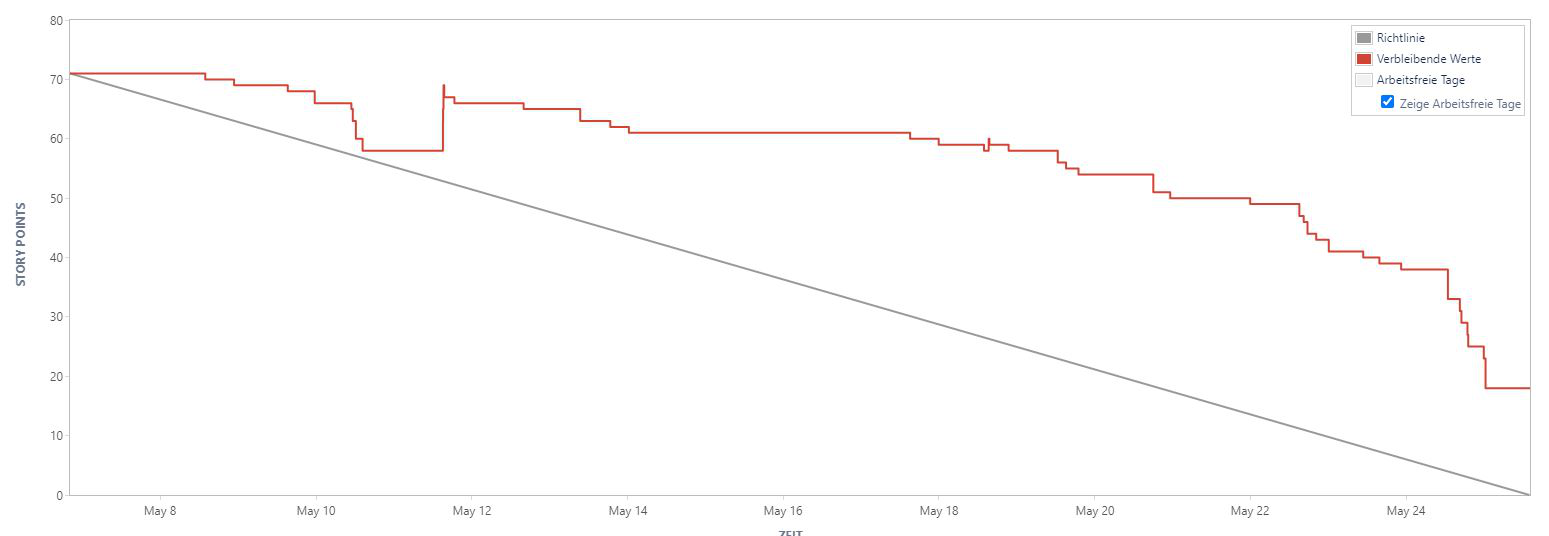
\includegraphics[width=\textwidth, height=5cm]{../img/sprint_10/Burndown-Sprint10.png}
        \caption{Burndown-Diagramm Sprint 10}
        \label{fig: Burndown-Sprint 10}
    \end{figure}

    \noindent
    Am Sprintbeginn betrug der Gesamtaufwand des Sprints 72 Story Points. Einige Tasks wurden frühzeitig fertiggestellt, sodass wir folgende Tasks nachgezogen haben:

    \begin{itemize}

        \item SWP2020A-36: ANmi, dass ich optional meiner Partie eine zufallsbasierte KI hinzufügen kann (5 Story Points)

        \item SWP2020A-233: ANmi bei einigen Aktionen und Events einfache Soundeffekte hören können(3 Story Points)

        \item SWP2020A-340: IllegalArgumentException beim Kauf einer Entwicklungskarte(1 Story Point)

        \item SWP2020A-341: ANmi bei einer Handelsnachricht im Chat immer nur die tatsächlich getauschten Ressourcen sehen können (1 Story Points)

        \item SWP2020A-342: Spiel-Canvas immer noch sichtbar nachdem man bereits gewonnen hat (1 Story Point)

        \item SWP2020A-343: Serverinterne Messages sollten nicht im DevMenu auftauchen (1 Story Point)

        \item SWP2020A-350: AEmi, dass Bamboo das Servermodul immer auf den Uniserver deployed, wenn der develop-Branch aktualisiert wird (2 Story Points)

    \end{itemize}

    \newpage
    \noindent
    Aus dem Burndown-Diagramm wird ersichtlich, dass im frühen Verlauf des Sprints die einige Tasks zügig abgeschlossen wurden vom Team, womit wir sehr nah an der Guideline des ganzen Sprints waren. Demnach wurden Tasks nachgezogen für die Teammitglieder, welche keine Tasks mehr hatten.
    Somit wurde die Gesamtanzahl von 72 Story Points auf 84 Story Points erhöht.
    Jedoch wird aus dem Burndown-Diagramm auch ersichtlich, dass nach dem Nachziehen der Tasks die Arbeitsaktivität relativ gering war. In der 2. Woche des Sprints wurden die Tasks nur langsam erledigt und die meisten Pull-Requests wurden gegen Ende des Code-Freezes gestellt. Des Weiteren wurden folgende Tasks nicht erfolgreich abgeschlossen bis zum Sprintende:

    \begin{itemize}

        \item SWP2020A-194 User und Author Objekt aus Messages entfernen und stattdessen "Message.getSession().get().getUser()" nutzen (2 Story Points)

        \item SWP2020A-205 ANmi, nachdem ich mind. 2 Züge verpasst habe (AFK), aus dem Spiel entfernt und durch eine KI ersetzt werden (2 Story Points)

        \item SWP2020A-256 ANmi statt der config.properties ein Einstellungsmenü nutzen können (4 Story Points)

        \item SWP2020A-292 Bericht für Sprint 09 erstellen (2 Story Points)

        \item SWP2020A-330 ANmi, dass die Dummies in der Gründerphase ihre Startsiedlungen und -straßen bauen (3 Story Points)

        \item SWP2020A-339 AEmi, dass die Phasen eines Spielzuges klar organisiert sind und ich angenehm damit arbeiten kann (5 Story Points)

    \end{itemize}

    \noindent
    Im gesamten Sprint wurden also nur 66 von 84 Story Points abgeschlossen.

    \newpage

    \subsection{Sprintprobleme bzw. Hindernisse}
    Das Team hatte nach der 2. Sprintwoche keine ersichtlichen Sprintfortschritte vorzuzeigen. Vom Team wurde viel prokrastiniert und viele Tasks wurden erst spät angefangen, sodass viele Pull-Requests erst sehr spät gestellt bzw. einige Tasks sogar gar nicht in PR gestellt wurden. Des Weiteren wurden teilweise unvollständige Tasks in PR gestellt, um somit den Code-Freeze zu umgehen. Jedoch zerstört diese Vorgehensweise den Sinn des Code-Freezes.
    Weiterhin wurde in diesem Sprint ersichtlich, dass einige Reviews langsam vorangegangen sind, welches zu einer Anstauung von PRs zum Ende des Sprints führte.

    \section{Erkenntnis aus der Retrospektive}
    Folgende Erkenntnisse ergaben sich aus der Retrospektive:\\

    \underline{Start:}
    \begin{itemize}
        \item Kummerkasten nutzen (!post)
        \item Früh anfangen
        \item Frühzeitige Bearbeitung
        \item Fortschritt im Meeting besprechen
    \end{itemize}

    \underline{Stop:}
    \begin{itemize}
        \item BEWEG DEINEN ARSCH
        \item Nur vollständige Tasks in PR stellen
        \item Keine funktional unvollständige PRs stellen
        \item Tasks gründlich und gewissenhaft bearbeiten
    \end{itemize}

    \underline{Weiter so:}
    \begin{itemize}
        \item Kleine Tasks geeignet für Solo-Programming
        \item Kommunikation ist TOP
        \item Solo
    \end{itemize}

    \newpage


    \section{Sonstige Anmerkungen}
    Was grundsätzlich anzumerken ist in diesem Sprint, ist die späte Bearbeitung von Tasks, welches dazu führte, dass viele PRs sich auf den letzten Drücker anstauen und somit viel Stress entsteht gegen Sprintende.
    Außerdem war die Höhe von Story Points in Sprint 10 (84 Story Points) beträchtlich höher als in den letzten beiden Sprints (Sprint 8: 36 Story Points und Sprint 9: 54 Story Points).
    Des Weiteren ist die Nachfrage nach Hilfe weiterhin möglich und auch erwünscht, sollte eine Person auf Probleme stoßen, die sie vorerst nicht allein bewältigen kann.


    \section{Fazit}
    Abschließend kann man erfassen, dass das Sprintziel \glqq Polishing des Projekts \grqq{} größtenteils erreicht wurde. Es wurden viele Bugs behoben und allerlei Dinge verbessert. Im Folgenden sollten während der Meetings der Fortschritt der eigenen Tasks genauer besprochen werden, damit sich am Sprintende nicht zu viele Tasks anstauen bzw. gar nicht erst bearbeitet werden. Des Weiteren sollte das Team versuchen sich so gut wie möglich an der Guideline des Burndown-Diagramms zu halten, um einen stetigen und einwandfreien Sprintverlauf zu erzielen.

\end{document}